\section{系统架构与模块}

\subsection{使用的平台和技术}

\begin{itemize}
\item[-]Linux
 
Linux是高性能的开源操作系统,在服务器环境上有着非常广泛的应用,很多开源的程序和平台都是基于Linux的。

Linux是OJ的的开发和部署平台,虽然Python可以跨平台,但是在Windows上兼容性并不好,同时因为很多系统API的不一致,部分运行库并没有兼容Windows或者Windows上运行效率比较低。

\item[-]Python和Django
 
Python是一种面向对象的脚本语言,语法简洁易读,具有丰富和强大的类库,而且和C/C++语言进行混合编程非常方便。本OJ的判题沙箱就是使用C语言编写的,然后与Python混合调用。

Django是本项目使用的Web框架,是最著名的Python Web框架。使用Django可以让你比较小的代价来构建和维护高质量的Web应用。
    
\item[-]MySQL和Redis
 
MySQL是关系型数据库,是OJ中数据存储的主力。因为它开源、性能高等特点,已经成为最流行的数据库,广泛的用在互联网上各种网站上。

Redis是内存数据库,主要用于Key-Value类型数据的存储,存取速度非常快。担当队列和缓存的角色。

\item[-]Docker
 
Docker是一个应用容器引擎,和虚拟机相比,更加轻量级和易用。开发者可以创建Docker镜像,让代码在容器中运行,方便发布到多台服务器上。OJ用Docker来创建测试和部署环境,大大简化了部署过程。

\item[-]Bootstrap

Bootstrap是来自Twitter的前端框架,包括HTML、CSS和JavaScript框架,提供排版、表单、按钮、导航等各种组件。它简洁灵活,使得Web开发更加快捷。

\item[-]avalon
 
avalon是OJ使用的前端MVVM框架。在传统前端开发中,很多动态的效果需要拼接HTML然后直接进行DOM操作,这是造成JavaScript代码无法维护的元凶之一,使用MVVM框架可以不再手动的去操作DOM,简化了操作,而且可以提高性能。类似的框架还有Vue.js和Angular JS。
    
\item[-]MVC和RESTful API
 
MVC是一种软件架构模式,分为三部分:Model、View和 Controller。Django就是一个MVC的框架,数据库定义在Model中,View是业务逻辑,Controller就是框架本身。Django将不同的URL和View进行绑定,然后传递到View中指定的函数进行处理。

前端JavaScript和后端的Python代码使用RESTful API进行通信,数据格式是JSON。这样实现了复杂页面的前后端分离。

\end{itemize}

\subsection{系统架构与组成}

OJ系统后端由MySQL数据库、Redis、异步队列、判题服务器、测试用例同步模块组成,其中,OJ系统将用户提交的代码和判题信息存储在一个单独的MySQL数据库中,用户信息和题目等在另外一个数据库中。

多数情况下,系统只需要使用ORM与MySQL数据库进行交互,进行增删改查,然后渲染前端模板显示。比较复杂的流程是判题流程,用户提交代码后,写入数据库,创建判题任务并交给异步队列去处理,立即返回前端提交id,前端定时使用提交id来获取提交状态并提示用户。异步队列根据当前系统设置调度选择一台判题服务器,调用RPC接口发送用户代码、题目信息等数据,判题服务器编译运行用户代码并返回给Web服务器运行结果然后更新数据库。系统还可能进行的操作包括:更新题目计数器、更新用户做题状态、更新比赛排名、更新用户排名和部分缓存的主动失效等。

\begin{figure}[H]
\centering
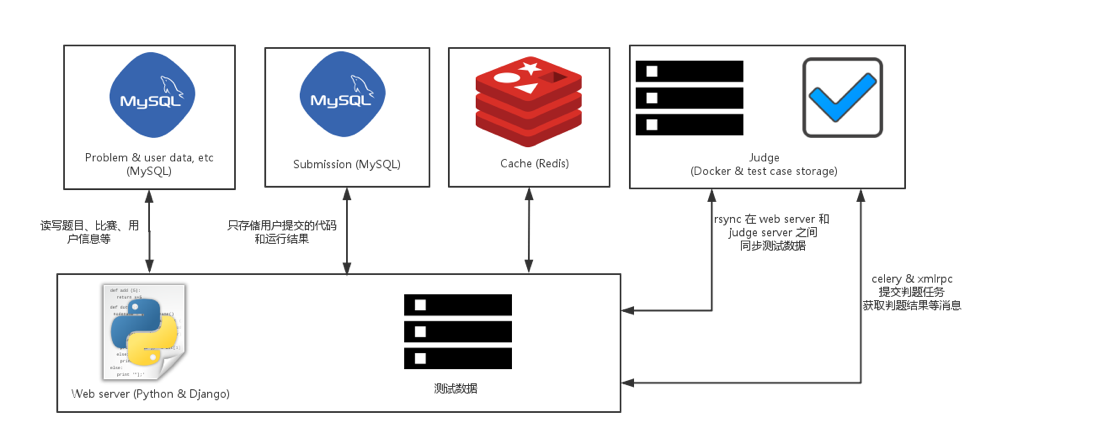
\includegraphics[width=0.9\textwidth]{oj-structures}
\caption{OJ后端架构图}
\end{figure}

Web前端使用了Bootstrap作为前端UI框架,使用了avalon作为 MVVM框架。由于JavaScript数量非常多,依赖关系也很复杂,所以还使用了require.js进行JavaScript模块化,使用了r.js进行静态文件的压缩和合并。

\subsection{功能模块}

\begin{figure}[H]
\centering
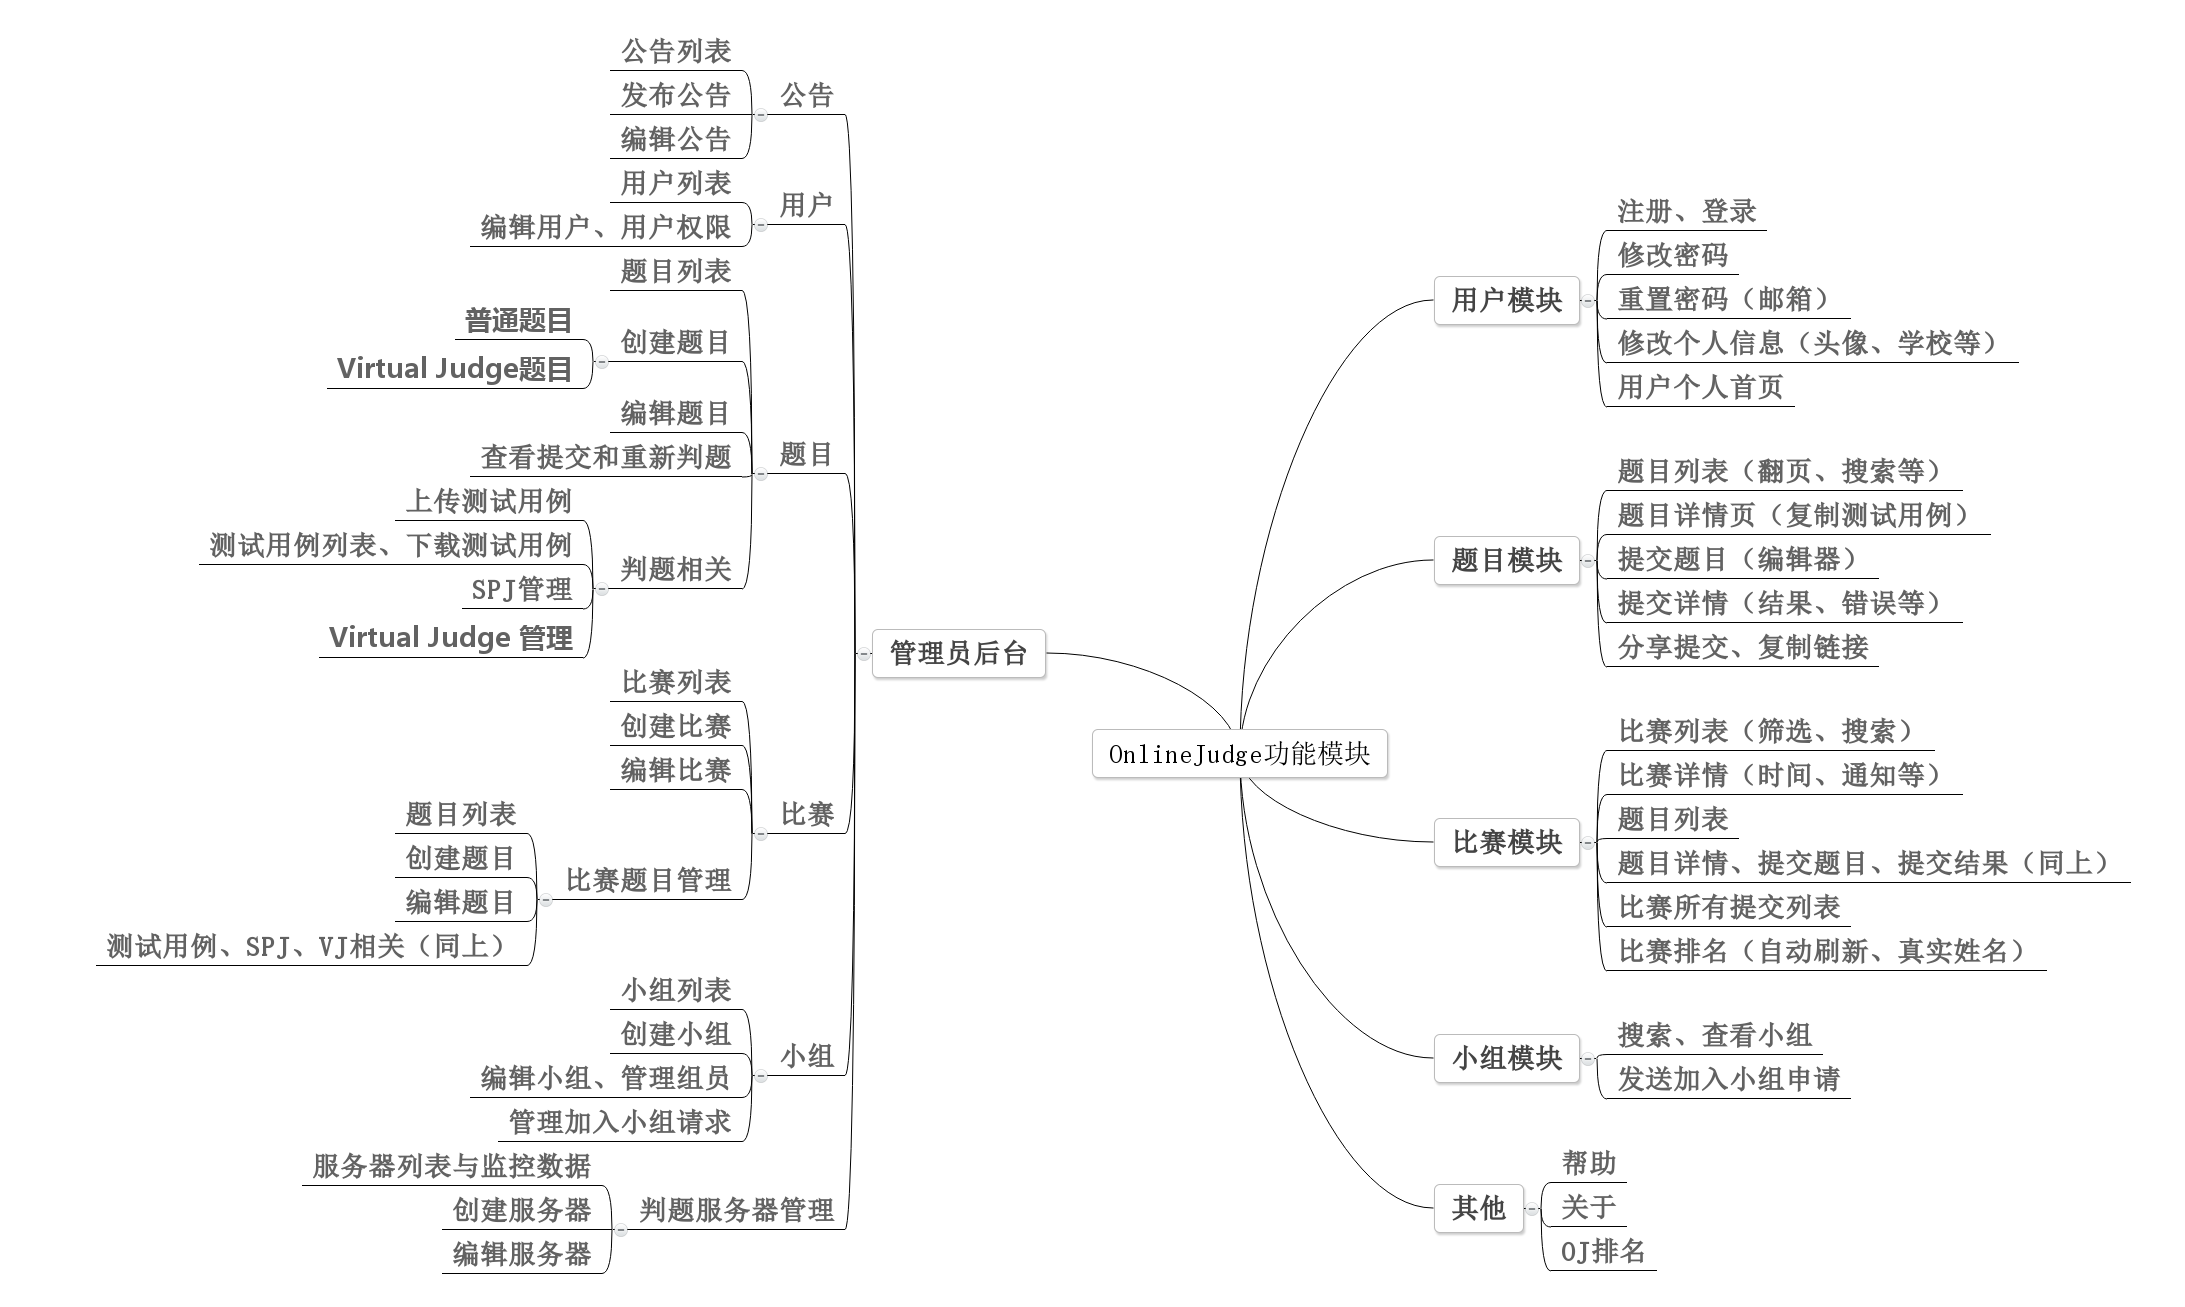
\includegraphics[width=\textwidth]{OJ-module}
\caption{OJ功能模块}
\end{figure}

